\documentclass[a4paper,11pt]{report}
\usepackage{chuan_math_gkt}
\usetikzlibrary{angles,quotes,intersections,patterns,decorations.pathreplacing}
\chuanexamsetup

\begin{document}
\examfontsize

\examsecret{绝密$\bigstar$启用前}

\examtitle{2022年普通高等学校招生全国统一考试（新高考II卷）}{数\quad 学}

\noticetitle
\begin{examnotice}
\item 答卷前，考生务必将自己的姓名、准考证号填写在答题卡上. 
\item 回答选择题时，选出每小题的答案后，用铅笔把答题卡上对应题目的答案标号涂黑. 如需改动，用橡皮擦干净后，再选涂其他答案标号. 回答非选择题时，将答案写在答题卡上. 写在本试卷上无效. 
\item 考试结束后，将本试卷和答题卡一并交回. 
\end{examnotice}

\examsection{一、选择题：本题共8小题，每小题5分，共40分. 在每小题给出的四个选项中，只有一项是符合题目要求的. }
\begin{examquestions}
\item 已知集合 $A=\{-1,1,2,4\}$，$B=\{x\mid |x-1|\leq1\}$，则 $A\cap B=$
\fourchoices{$\{-1,2\}$}{$\{1,2\}$}{$\{1,4\}$}{$\{-1,4\}$}
\item $(2+2\mathrm{i})(1-2\mathrm{i})=$
\fourchoices{$-2+4\mathrm{i}$}{$-2-4\mathrm{i}$}{$6+2\mathrm{i}$}{$6-2\mathrm{i}$}
\item 图1是中国古代建筑中的举架结构，$AA',BB',CC',DD'$ 是桁，相邻桁的水平距离称为步，垂直距离称为举；图2是某古代建筑屋顶截面的示意图. 其中 $DD_1,CC_1,BB_1,AA_1$ 是举，$OD_1,DC_1,CB_1,BA_1$ 是相等的步，相邻桁的举步之比分别为 $\dfrac{DD_1}{OD_1}=0.5$，$\dfrac{CC_1}{DC_1}=k_1$，$\dfrac{BB_1}{CB_1}=k_2$，$\dfrac{AA_1}{BA_1}=k_3$. 已知 $k_1,k_2,k_3$ 成公差为0.1的等差数列，且直线 $OA$ 的斜率为0.725，则 $k_3=$
\begin{tightcenter}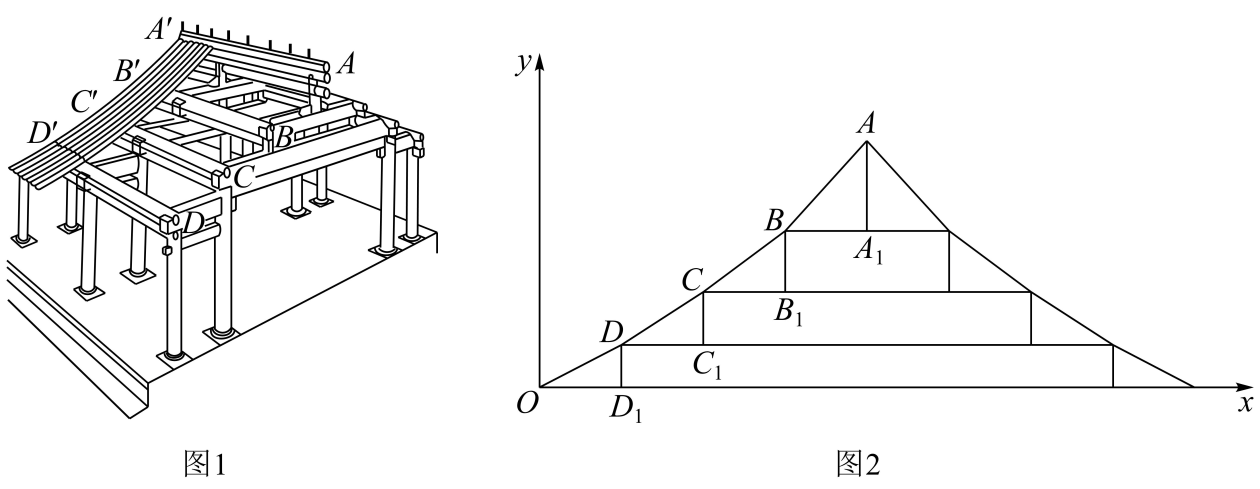
\includegraphics[width=10.0cm]{figures/2022_xgk2_q3.png}\end{tightcenter}
\fourchoices{$0.75$}{$0.8$}{$0.85$}{$0.9$}
\item 已知向量 $\vec a=(3,4)$，$\vec b=(1,0)$，$\vec c=\vec a+t\vec b$，若 $\langle\vec a,\vec c\rangle=\langle\vec b,\vec c\rangle$，则 $t=$
\fourchoices{$-6$}{$-5$}{$5$}{$6$}
\item 有甲、乙、丙、丁、戊5名同学站成一排参加文艺汇演，若甲不站在两端，丙和丁相邻，则不同排列方式共有
\fourchoices{12种}{24种}{36种}{48种}
\item 若 $\sin(\alpha+\beta)+\cos(\alpha+\beta)=2\sqrt2\cos\left(\alpha+\dfrac\pi4\right)\sin\beta$，则
\twochoices{$\tan(\alpha-\beta)=1$}{$\tan(\alpha+\beta)=1$}{$\tan(\alpha-\beta)=-1$}{$\tan(\alpha+\beta)=-1$}
\item 已知正三棱台的高为1，上、下底面边长分别为 $3\sqrt3$ 和 $4\sqrt3$，其顶点都在同一球面上，则该球的表面积为
\fourchoices{$100\pi$}{$128\pi$}{$144\pi$}{$192\pi$}
\item 已知函数 $f(x)$ 的定义域为 $\mathbb R$，且 $f(x+y)+f(x-y)=f(x)f(y)$，$f(1)=1$，则 $\sum_{k=1}^{22}f(k)=$
\fourchoices{$-3$}{$-2$}{$0$}{$1$}
\end{examquestions}
\examsection{二、选择题：本题共4小题，每小题5分，共20分. 在每小题给出的选项中，有多项符合题目要求. 全部选对的得5分，部分选对的得2分，有选错的得0分. }
\begin{examquestions}[start=9]
\item 已知函数 $f(x)=\sin(2x+\varphi)(0<\varphi<\pi)$ 的图像关于点 $\left(\dfrac{2\pi}{3},0\right)$ 中心对称，则
\onechoices{\tallchoice{$f(x)$ 在区间 $\left(0,\dfrac{5\pi}{12}\right)$ 单调递减}}{\tallchoice{$f(x)$ 在区间 $\left(-\dfrac\pi{12},\dfrac{11\pi}{12}\right)$ 有两个极值点}}{\tallchoice{直线 $x=\dfrac{7\pi}{6}$ 是曲线 $y=f(x)$ 的对称轴}}{\tallchoice{直线 $y=\dfrac{\sqrt3}{2}x$ 是曲线 $y=f(x)$ 的切线}}
\item 已知 $O$ 为坐标原点，过抛物线 $C:y^2=2px(p>0)$ 焦点 $F$ 的直线与 $C$ 交于 $A,B$ 两点，其中 $A$ 在第一象限，点 $M(p,0)$，若 $|AF|=|AM|$，则
\twochoices{直线 $AB$ 的斜率为 $2\sqrt6$}{$|OB|=|OF|$}{$|AB|>4|OF|$}{$\angle OAM+\angle OBM<180^\circ$}
\item 如图，四边形 $ABCD$ 为正方形，$ED\perp$ 平面 $ABCD$，$FB\parallel ED$，$AB=ED=2FB$，记三棱锥 $E-ACD$，$F-ABC$，$F-ACE$ 的体积分别为 $V_1,V_2,V_3$，则

\noindent\begin{minipage}[t]{0.62\linewidth}
\twochoices{$V_3=2V_2$}{$V_3=V_1$}{$V_3=V_1+V_2$}{$2V_3=3V_1$}
\end{minipage}\hfill
\begin{minipage}[t]{0.23\linewidth}\vspace{-1.6em}\centering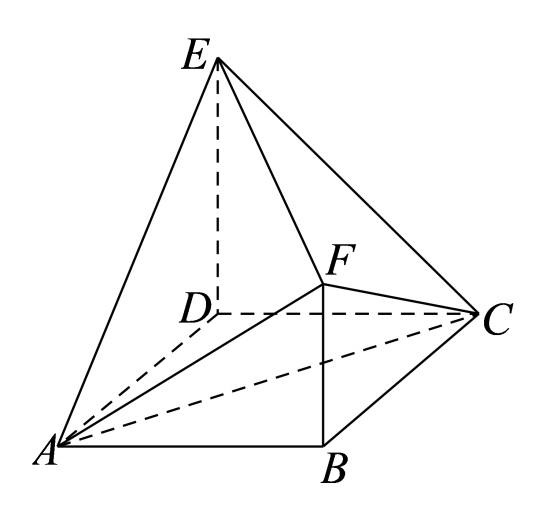
\includegraphics[width=\linewidth]{figures/2022_xgk2_q11.png}\end{minipage}
\item 若 $x,y$ 满足 $x^2+y^2-xy=1$，则
\twochoices{$x+y\leq1$}{$x+y\geq-2$}{$x^2+y^2\leq2$}{$x^2+y^2\geq1$}
\end{examquestions}
\examsection{三、填空题：本题共4小题，每小题5分，共20分. }
\begin{examquestions}[start=13]
\item 已知随机变量 $X$ 服从正态分布 $N(2,\sigma^2)$，且 $P(2<X\leq2.5)=0.36$，则 $P(X>2.5)=\blank$. 
\item 曲线 $y=\ln|x|$ 过坐标原点两条切线的方程为\blank，\blank. 
\item 设点 $A(-2,3),B(0,a)$，若直线 $AB$ 关于 $y=a$ 对称的直线与圆 $(x+3)^2+(y+2)^2=1$ 有公共点，则 $a$ 的取值范围是\blank. 
\item 已知直线 $l$ 与椭圆 $\dfrac{x^2}{6}+\dfrac{y^2}{3}=1$ 在第一象限交于 $A,B$ 两点，$l$ 与 $x$ 轴、$y$ 轴分别交于 $M,N$ 两点，且 $|MA|=|NB|,|MN|=2\sqrt3$，则 $l$ 方程为\blank. 
\end{examquestions}
\examsection{四、解答题：本题共6小题，共70分. 解答应写出文字说明，证明过程或演算步骤. }
\begin{examanswers}[start=17]
\item（10分）

已知 $\{a_n\}$ 为等差数列，$\{b_n\}$ 是公比为2的等比数列，且 $a_2-b_2=a_3-b_3=b_4-a_4$. 

（1）证明：$a_1=b_1$；

（2）求集合 $\{k\mid b_k=a_m+a_1,1\leq m\leq500\}$ 中元素个数. 
\item（12分）

记 $\triangle ABC$ 的内角 $A,B,C$ 的对边分别为 $a,b,c$，分别以 $a,b,c$ 为边长的三个正三角形的面积依次为 $S_1,S_2,S_3$，已知 $S_1-S_2+S_3=\dfrac{\sqrt3}{2}$，$\sin B=\dfrac13$. 

（1）求 $\triangle ABC$ 的面积；

（2）若 $\sin A\sin C=\dfrac{\sqrt2}{3}$，求 $b$. 
\newpage
\item（12分）

在某地区进行流行病学调查，随机调查了100位某种疾病患者的年龄，得到如下的样本数据的频率分布直方图：
\begin{tightcenter}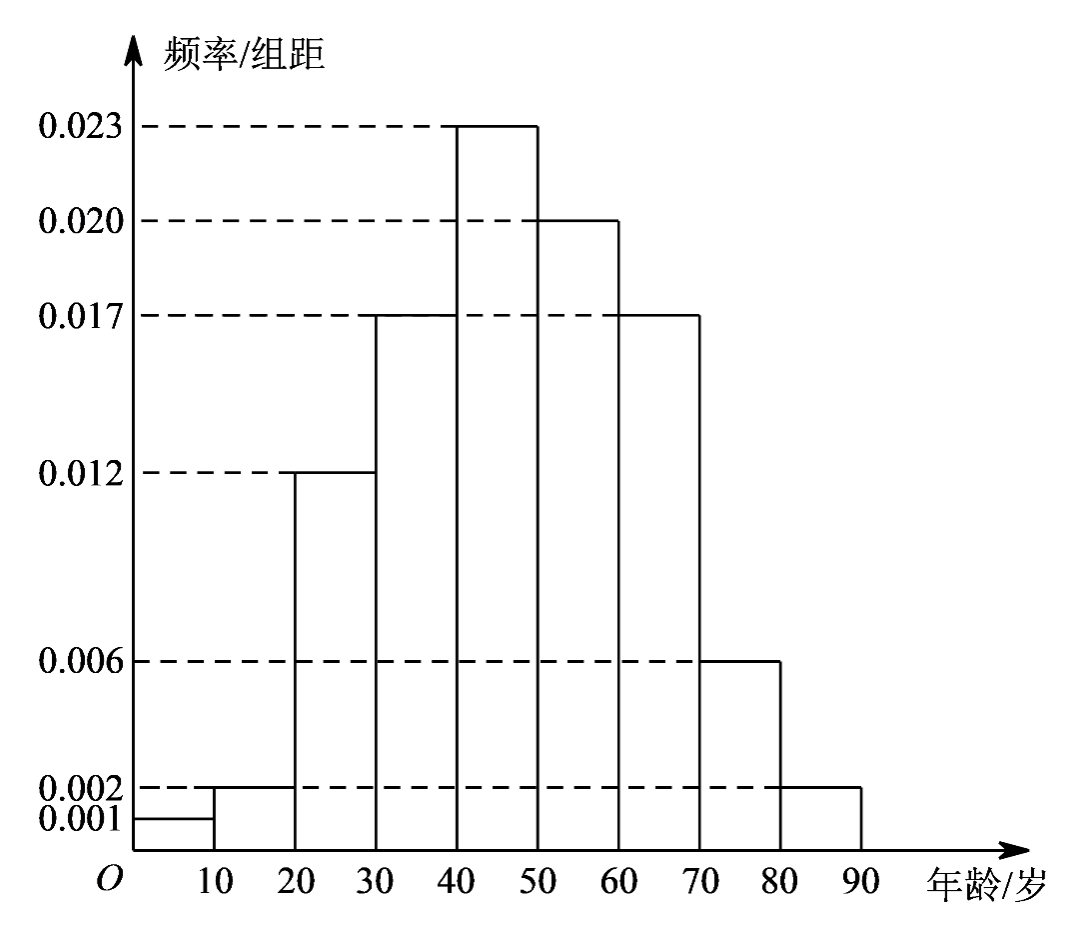
\includegraphics[width=7.2cm]{figures/2022_xgk2_q19.png}\end{tightcenter}
（1）估计该地区这种疾病患者平均年龄（同一组中的数据用该组区间的中点值为代表）；

（2）估计该地区一位这种疾病患者的年龄位于区间 $[20,70)$ 的概率；

（3）已知该地区这种疾病的患病率为 $0.1\%$，该地区年龄位于区间 $[40,50)$ 的人口占该地区总人口的 $16\%$. 从该地区中任选一人，若此人的年龄位于区间 $[40,50)$，求此人患这种疾病的概率. （以样本数据中患者的年龄位于各区间的频率作为患者的年龄位于该区间的概率，精确到0.0001）
\item（12分）

如图，$PO$ 是三棱锥 $P-ABC$ 的高，$PA=PB$，$AB\perp AC$，$E$ 是 $PB$ 的中点. 

\noindent\begin{minipage}[t]{0.62\linewidth}
（1）证明：$OE\parallel$ 平面 $PAC$；

（2）若 $\angle ABO=\angle CBO=30^\circ$，$PO=3$，$PA=5$，求二面角 $C-AE-B$ 的正弦值. 
\end{minipage}\hfill
\begin{minipage}[t]{0.32\linewidth}\vspace{-1.2em}\centering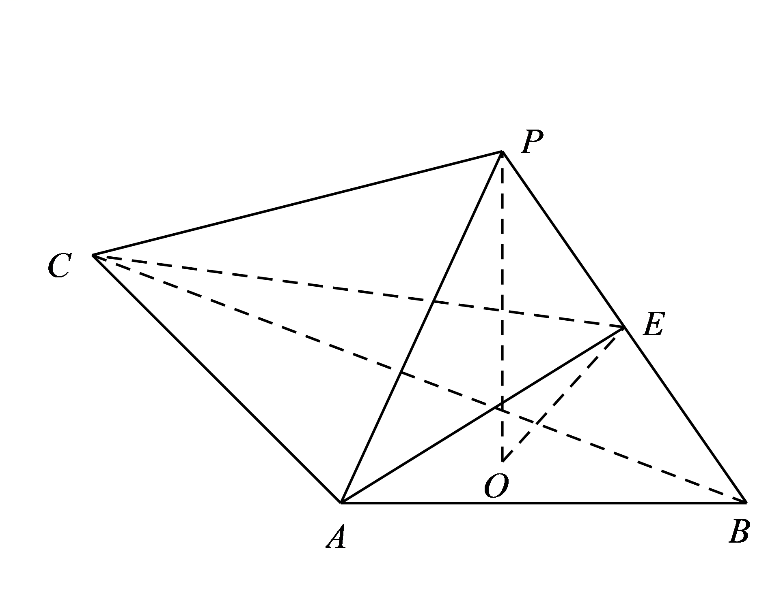
\includegraphics[width=\linewidth]{figures/2022_xgk2_q20.png}\end{minipage}
\newpage
\item（12分）

已知双曲线 $C:\dfrac{x^2}{a^2}-\dfrac{y^2}{b^2}=1(a>0,b>0)$ 的右焦点为 $F(2,0)$，渐近线方程为 $y=\pm\sqrt3x$. 

（1）求 $C$ 的方程；

（2）过 $F$ 的直线与 $C$ 的两条渐近线分别交于 $A,B$ 两点，点 $P(x_1,y_1),Q(x_2,y_2)$ 在 $C$ 上，且 $x_1>x_2>0,y_1>0$. 过 $P$ 且斜率为 $-\sqrt3$ 的直线与过 $Q$ 且斜率为 $\sqrt3$ 的直线交于点 $M$. 从下面①②③中选取两个作为条件，证明另外一个成立：

①$M$ 在 $AB$ 上；②$PQ\parallel AB$；③$|MA|=|MB|$. 

注：若选择不同的组合分别解答，则按第一个解答计分. 
\item（12分）

已知函数 $f(x)=xe^{ax}-e^x$. 

（1）当 $a=1$ 时，讨论 $f(x)$ 的单调性；

（2）当 $x>0$ 时，$f(x)<-1$，求 $a$ 的取值范围；

（3）设 $n\in\mathbb N^*$，证明：$\dfrac1{\sqrt{1^2+1}}+\dfrac1{\sqrt{2^2+2}}+\cdots+\dfrac1{\sqrt{n^2+n}}>\ln(n+1)$. 
\end{examanswers}

\end{document}
